\chapter{Elements of Quantum Computing}

We mentioned in the previous chapter that computer are electronic systems that process binary information
is the form of voltages, thus these systems are governed by the macroscopic laws of 
Classical Mechanics. But as they shurnk down to the microscopic levels of the atoms,
new problems arose. By manipulating and storing information in atoms, electrons, spins
and \textit{quantum systems} in general, now the computer itself must obey the laws
of Quantum Mechanic, a notion that Richard Feynman introduced in the early '80s.

\section{The Dirac Notation}

We already are familiar with the standard vector notation. Let $\vec{v}$ be a $n$-dimensional vector
whom's elements are real numbers. This is notated as:

\begin{equation}
    \vec{v}=\sum_{i=1}^{n}v_i\hat{d_i}\in\mathbb{R}^n
\end{equation}

where $\hat{d_i}$ is the unit vector of the $i$-th dimension. For a three-dimensional
real space the vector $\vec{v}$ would be notated as:

\begin{equation}
    \vec{v}=v_1\hat{d_1}+v_2\hat{d_2}+v_3\hat{d_3}\in\mathbb{R}^3
\end{equation}

The notation is similar for elements in the complex space $\mathbb{C}^n$. The only real difference
is the nomenclature where vectors that are in that space are called \textit{complex vectors}.

We can also notate vectors as a $n\times1$ column matrix, where each element of that matrix
is the vector's corresponding element:

\begin{equation}
    \vec{v}=\begin{bmatrix}
        v_1\\
        v_2\\
        \vdots\\
        v_n
    \end{bmatrix}\in\mathbb{R}^n
\end{equation}

In Quantum Mechanics, vectors are represented using a different kind of notation, the \textit{Dirac notation}
or \textit{bra-ket notation}. This notation was introduced by the American physicist and electrical engineer Paul
Dirac in 1939 \cite{Dirac1939}. This introduced two new symbols: the \textit{bra} (symbolised with a $\bra{}$)
which represents a vector quantity whose elements are a vertical $1\times n$ matrix, and the \textit{ket}
(symbolised with a $\ket{}$) which represents a vector quantity whose elements are a horizontal $n\times1$ matrix.
We also note that in Quantum Mechanics all vectors (and their elements) are in a complex space. For example,
let $\vec{v}$ be a vector in the complex space $\mathbb{V}^n$, we would notate it in Dirac notation as:

\begin{equation}
    \ket{v}=\begin{bmatrix}
        v_1\\
        v_2\\
        \vdots\\
        v_n
    \end{bmatrix}
    \text{, where }v_i\in\mathbb{C},\ket{v}\in\mathbb{V}^n
\end{equation}
This is also read as \say{ket $v$}. Note that the arrow symbol ($\rightarrow$) on top of label-name of the vector
$\vec{v}$ is absent with this notation.

Subsequently, the \say{bra $v$} is the \textit{conjugate transpose} or the \textit{Hermitian conjugate} (symbolised with
$\dag$ and pronounced as \say{dagger}) of the $\ket{v}$

\begin{equation}
    \bra{v}=\begin{bmatrix}
        v_1^*&v_2^*&\hdots&v_n^*
    \end{bmatrix}=
    \begin{bmatrix}
        v_1\\
        v_2\\
        \vdots
        v_n
    \end{bmatrix}^\dag
\end{equation}

\subsection{Inner Product}

The inner product of two complex vectors $\ket{a},\ket{b}\in\mathbb{V}^n$ is defined as

\begin{equation}
    \braket{a|b}=\begin{bmatrix}
        a_1^*&a_2^*\hdots a_n^*
    \end{bmatrix}\times
    \begin{bmatrix}
        b_1\\
        b_2\\
        \vdots\\
        b_n
    \end{bmatrix}=
    \sum_{i=1}^{n}a_i^*b_i=c\text{, where }a_i,b_i,c\in\mathbb{C}
\end{equation}

There are also three properties defined for the inner product:

\begin{equation}
    \braket{a|b}=\braket{b|a}^*
\end{equation}

\begin{equation}
    \braket{a|\alpha b+\beta c}=\alpha\braket{a|b}+\beta\braket{a|c}\text{, where }\alpha,\beta\in\mathbb{C}
\end{equation}

\begin{equation}
    \braket{\alpha a+\beta c|b}=\alpha^*\braket{a|b}+\beta^*\braket{c|a}\text{, where }\alpha,\beta\in\mathbb{C}
\end{equation}

The inner product of two vectors $\ket{a},\ket{b}\in\mathbb{V}^n$ is zero when the vectors are orthogonal to each other.

\subsection{Hilbert Space}

When in an abstract complex vector space $\mathbb{V}^n$ the operation of the inner product is defined then
that space is also called a \textit{Hilbert space}. In Quantum Computing, every vector that represents the
state of the quantum system is a vector in Hilbert space.
\section{Operators}

In Quantum Mechanics, operators are mathematical objects that act on vectors and transform them.
The action of an operator, let $\hat{A}$ be an operator and $\ket{\phi}$ a qubit, is a expressed as:

\begin{equation}
    \hat{A}\ket{\phi}=\ket{\phi'}
\end{equation}

There are also defined properties for operators. Two operators $\hat{A},\hat{B}$ are equal when:

\begin{equation}
    \hat{A}\ket{\phi}=\hat{B}\ket{\phi}
\end{equation}

Addition between two operators $\hat{A},\hat{B}$ is defined as:

\begin{equation}
    (\hat{A}+\hat{B})\ket{\phi}=\hat{A}\ket{\phi}+\hat{B}\ket{\phi},\forall\ket{\phi}\in\mathbb{H}^n
\end{equation}

The product of two operators $\hat{A},\hat{B}$ defines the order of operations that act on a certain vector $\ket{\phi}$ as:

\begin{equation}
    \hat{A}\hat{B}\ket{\phi}=\hat{A}(\hat{B}\ket{\phi})=\hat{A}\ket{\phi'}
\end{equation}

We should note that the addition of two operators is commutative $\hat{A}+\hat{B}=\hat{B}+\hat{A}$ but that
does not apply in general to the product of two operators $\hat{A}\hat{B}\neq\hat{B}\hat{A}$.

\section{Matrices of Operators}

It is often simpler to represent the transformations of an operator using a matrix representation. Each element of that
matrix represents the transformation on a specific basis. For example, let $\hat{A}$ be an operator and $\{\ket{i}\},i=1,2,\hdots n$
be a basis in a Hilbert space $\mathbb{H}^n$, the operator can be represented as $n\times n$ matrix:

\begin{equation}
    \hat{A}=\begin{bmatrix}
        A_{11} & A_{12} & \hdots & A_{1n}\\
        A_{21} & A_{22} & \hdots & A_{2n}\\
        \vdots & \vdots & \ddots & \vdots\\
        A_{n1} & A_{n2} & \hdots & A_{nn}\\
    \end{bmatrix}
\end{equation}

There are many operators that are useful in Quantum Mechanics (and in extension also in Quantum Computing).

For example, the Identity operator, notated with an $\hat{I}$, is an operator that when applied on any vector $\ket{\phi}$
lefts it un-transformed:

\begin{equation}
    \hat{I}\ket{\phi}=\ket{\phi}
\end{equation}

and is represented as:

\begin{equation}
    \hat{I}=\begin{bmatrix}
        1 & 0 & \hdots & 0\\
        0 & 1 & \hdots & 0\\
        \vdots & \vdots & \ddots & \vdots\\
        0 & 0 & \hdots & 1\\
    \end{bmatrix}
\end{equation}

\section{Hermitian Conjugate}

Let $\ket{u}$ be a state vector of a quantum system and $\hat{A}$ be an operator that operates on $\ket{u}$:

\begin{equation}
    \hat{A}\ket{u} = \ket{u'}
\end{equation}

The same logic can be applied for its bra counterpart:

\begin{equation}
    \bra{u}\hat{A}^\dag = \bra{u'}
\end{equation}

where $\hat{A}^\dag$ is the \textit{Hermitian conjugate} of the operator $\hat{A}$ - its an operator
that when operated on $\bra{u}$ results in $\bra{u'}$ just like when its non-Hermitian conjugate
$\hat{A}$ operates on $\ket{u}$ and results in $\ket{u'}$.

Thus, when we take the conjugate of $\hat{A}^\dag$ then:

\begin{equation}
    (\hat{A}^\dag)^\dag=\hat{A}
\end{equation}

The matrix of $\hat{A}^\dag$ is defined as the \textit{conjugate transpose} matrix of the operator $\hat{A}$:

\begin{equation}
    \hat{A}^\dag=(\hat{A}^T)^*
\end{equation}

where $\hat{A}^T$ is the \textit{transpose} matrix of $\hat{A}$ and it is defined as:

\begin{equation}
    \hat{A}_{ij}^T=\hat{A}_{ji}
\end{equation}
\section{Quantum Mechanics for Quantum Computing}

Before we begin to operate a quantum computer or make quantum circuits we have to discuss
what are the underline laws that govern those systems.

Quantum Mechanics is a mathematical framework that is used to create physical theories or
to describe properties of physical systems. It is also a framework that helps physicists
to describe nature at the microscopic level, something that Classical Mechanics failed to do.

This mathematical framework has four \textit{axioms} that are used to interconnect the physical
with the mathematical world.

\subsection{The Axioms of Quantum Mechanics}
\subsubsection{Axiom One: The State of a Quantum System}

The state of a quantum system can be represented as a complex vector, which vector is in the
complex Hilber space. The state of a quantum system is also called the \textit{state vector} of
that quantum system. In quantum computing usually systems are \textit{two level systems}, that are systems
that have two states (binary systems).

The \textit{qubit} is the quantum equivalent of the classical bit - instead of storing classical information
(zeros or ones) is stores quantum information expressed using some \textit{basis states}. The most frequent
state base is the \textit{computational basis}. The computational basis describes two linearly seperable
and orthogonal unitary vectors $\{\ket{0},\ket{1}\}\in\mathbb{H}^2$. With those two states we can encode
information and process it using quantum gates. Physicaly these two state have to represent
a physical state of the system. Classical computers use two voltage levels (+5V and +0V, for example), in 
quantum computers we can use many physical properties of a quantum system like: the spin of an
electron (up or down), the polarization of a photon (horizontal or vertical) or even the energy levels of an atom.

A general state $\ket{\phi}$ of a system can be written as a superposition of the basis states $\ket{0}$ and $\ket{1}$:

\begin{equation}
    \ket{\phi} = a\ket{0} + b\ket{1} = \begin{bmatrix}
        a\\
        b
    \end{bmatrix}
\end{equation}

where $a,b\in\mathbb{C}$ are the complex coefficients called the \textit{probability amplitudes} of
the state vector $\ket{\phi}$. We can also notate them using the name of the state vector

\begin{equation}
    \ket{\phi} = \phi_0\ket{0} + \phi_1\ket{1} = \begin{bmatrix}
        \phi_0\\
        \phi_1
    \end{bmatrix}
\end{equation}

\subsubsection{Axiom Two: Time Evolution of a Quantum System}

The time evolution of a quantum system $\ket{\phi(t)}$ can be expresed by unitary operators
of the form $U(t, t_0)$ as follows:

\begin{equation}
    \ket{\phi(t)} = U(t, t_0)\ket{\phi(t_0)}
\end{equation}

Also if an operator is hermitian ($A=A^\dag$) then the operator $U=e^{iA}$ is unitary because:

\begin{equation}
    UU^\dag=e^{iA}(e^{iA})^\dag=e^{iA}e^{-iA^\dag}=e^{iA}e^{-iA}=I
\end{equation}

\subsubsection{Axiom Three: Measurement}

By now we can encode information and we can define its evolution in time, but it would be
gratuitous if we could not measure the outcome of any computation. Thus the third axiom states
that to make a measurement on a quantum system $\ket{\phi}\in\mathbb{H}$, defined using the
basis state $\ket{i}\in\mathbb{H}$, then a measurement can occur on $\ket{\phi}=\sum_{i}^{n}a_i\ket{i}$.
The outcome is one of the states $\ket{i}$ of the system with a probability to be in that state $|a_i|^2$.
After the outcome, the system \textit{collapses} to the that state $\ket{i}$.

\subsubsection{Axiom Four: Composite Systems}

We can combine $n$ independent quantum systems that are expressed as state vectors $\ket{\phi_i}\in\mathbb{H}_i$ where
$i=0,1,\hdots,n$ as a \textit{composite quantum system} $\ket{\phi}$. This can be done by applying the tensor product
to each of the independent systems

\begin{equation}
    \ket{\phi} = \ket{\phi_0}\otimes\ket{\phi_1}\otimes\hdots\otimes\ket{\phi_n}=\ket{\phi_0\phi_1\hdots\phi_n}
\end{equation}

That state vector $\ket{\phi}$ is a complex vector in the complex Hilber space

\begin{equation}
    \mathbb{H}=\mathbb{H}_0\otimes\mathbb{H}_1\otimes\hdots\mathbb{H}_n
\end{equation}

As we mentioned previously, in Quantum Computing, we study two-level systems - systems with two basis states.
This means that the composite system $\ket{\phi}$ of $n$ independent two-level quantum systems
is in a complex Hilbert space of $2^n$ dimensions.
\section{Reversible Computation}

\say{Classical} computers use three fundamental logic gates to process binary information:
the AND, OR and NOT gates as we have introduced them in the previous chapter. A very simple
question can rise from analyzing these logic gate \say{Can we know the state of the inputs by
just looking at the outputs}? In other words, \say{Can we reverse the computation done by those
logic gates}?

The NOT gate is \textit{reversible} because its output is the negation of the input and we can infer
the input by just negating again. This is also a postulate of the Boolean Algebra:

\begin{equation}
    \lnot(\lnot x) = x
\end{equation}

The AND and OR gates are not reversible. For the AND gate, we have three outputs
that result in a zero (0) and only one possibility for an output of one (1), thus we cannot infer
for three outputs what the inputs are with absolute certainty. For the OR gate is the same
but instead of three outputs of zero this gate has three possibilities of outputs of one (1).
It seems like we lost some information of what the inputs were. In fact we do lose information
in form of heat \cite{Landauer1961}. We can analyze for the other compound gates: NAND, NOR, XOR
and XNOR. We can find out easily that all of those gate are not reversible for the same reasons.

The most important thing to consider is the energy loss in the form of heat. It has been shown \cite{Bennett1982}
that by making logic components reversible we can save a lot of power generated by the computer.
These kind of components are called \textit{reversible logic gates}. This idea of reversible computation
is the basis that Feynman used to impose the idea of the Quantum Computer, a computer that uses
reversible components that obey the laws of Quantum Mechanics \cite{Feynman1982}.
\section{Landauer's Principle}

When one bit of information is erased, the least amount of energy is expelled to the enviroment given by the
following equation:

\begin{equation}
    E = k_BT\ln2
\end{equation}

where $k_B$ is the \textit{Boltzmann constant} and $T$ is the temperature of the enviroment. This is
know as the \textit{Landauer's Principle}\cite{Landauer1961}. We can use this equation to calculate the total work produced
by the computer by defining a Boolean function $f:\{0,1\}^m\to\{0,1\}^n$ that takes $m$-input bits and
produces $n$-output bits - this funtion will represent all of the logical operations of the computer.
If we consider that $m>>n$, this means that some bits are erased each time the computer carries a computation\cite{Marmorkos2024},
then the total energy loss using equation (3.8) is:

\begin{equation}
    E_{total}=(m-n)k_BT\ln2
\end{equation}

Because Equation (3.9) gives the minimum amount of energy produced, the real amount of energy produced by
modern computers is much higher that $E_{total}$.
\section{The Qubit}

As we have already described in a previous section, qubits are the fundamental units of measuring
the information contents of a quantum system. In classical terms, computers use two voltage levels
to represent the two states of a bit: choosing arbitrarily, +0V for the zero state and +5V for the
one state. Quantum systems map those logical states of qubits to some physical property of the quantum
system, which can be its spin, for electrons, or its polarity, for photons. Mathematically we represent
those states (0 and 1) with the \textit{unit vectors} $\ket{0}$ and $\ket{1}$ which constitute the
computational basis.

These basis are complex vectors $\ket{0},\ket{1}\in\mathbb{H}^2$ and are written as:

\begin{align}
    \ket{0}=\begin{bmatrix}
        1\\
        0
    \end{bmatrix}
    \text{ and }
    &
    \ket{1}=\begin{bmatrix}
        0\\
        1
    \end{bmatrix}
\end{align}

The big difference from the classical bit is that qubits are a superposition of some two basis states.
Although this is a very interesting phenomenon, computation constitutes that at some point we would need
to output/read the result. We have to remind at this point that this would constitute a measurement and
the qubit would have to \say{collapse} to one of the two basis states with a probability equal to
the square of the probability amplitude of that basis state.

\subsection{The Bloch Sphere}

The Bloch sphere is an attempt to depict the state of qubit as a vector that originates from the center
of a sphere with a radius $r=1$.

Let $\ket{q}=q_0\ket{0}+q_1\ket{1}\in\mathbb{H}^2$ be a qubit with $q_0,q_1\in\mathbb{C}$ be
its probability amplitudes. We can parameterize those coefficients as:

\begin{align}
    q_0 = e^{i\gamma}\cos\frac{\theta}{2} &\hspace{2cm}
    q_1 = e^{i\delta}\sin\frac{\theta}{2}
\end{align}

We can now re-write the qubit $\ket{q}$ as:

\begin{equation}
    \ket{q}=e^{i\gamma}(\cos\frac{\theta}{2}\ket{0}+e^{i\phi}\sin\frac{\theta}{2}\ket{1})
\end{equation}

where $\phi=\gamma-\delta$. The \textit{global phase} $e^{i\gamma}$ is neglected most of the time
thus qubit $\ket{q}$ can be written as a matrix:

\begin{equation}
    \ket{q}=\begin{bmatrix}
        \cos\frac{\theta}{2}\\
        e^{i\phi}\sin\frac{\theta}{2}
    \end{bmatrix}
\end{equation}

To map the \emph{spherical coordinates} $(r,\phi,\theta)$ to cartesian coordinates we use the equalities:

\begin{gather}
    q_x=r\sin\theta\cos\phi\\
    q_y=r\sin\theta\sin\phi\\
    q_z=r\cos\theta
\end{gather}

So the qubit $\ket{q}$ can be plotted with coordinates $(q_x,q_y,q_z)$.

\begin{figure}[ht]
    \centering
    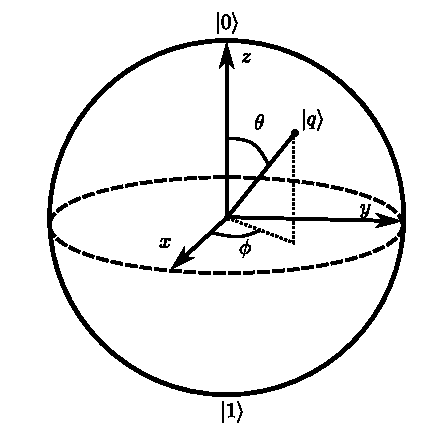
\includegraphics{images/3_Quantum_Computing/bloch_sphere.pdf}
    \caption{The Bloch sphere}
    \label{fig:bloch_sphere}
\end{figure}

We can note also the rest of the basis state that a qubit can have:

\begin{enumerate}
    \item along the $z$-axis we can distinguish the computational basis (see \ref{fig:bloch_sphere}): \begin{enumerate}
        \item $\ket{0}$ where the $+z$-axis crosses Bloch sphere's upper boundary
        \item $\ket{1}$ where the $-z$-axis crosses Bloch shpere's lower boundary
    \end{enumerate}
    \item along the $x$-axis: \begin{enumerate}
        \item at the cross section $+x$-axis where angles $\theta=\pi/2$ and $\phi=0$ we have the basis state $\ket{+}=\frac{\ket{0}+\ket{1}}{\sqrt{2}}$
        \item at the cross section $-x$-axis where angles $\theta=\pi/2$ and $\phi=\pi$ we have the basis state $\ket{-}=\frac{\ket{0}-\ket{1}}{\sqrt{2}}$
    \end{enumerate}
    \item along the $y$-axis: \begin{enumerate}
        \item at the cross section $+y$-axis where angles $\theta=\pi/2$ and $\phi=\pi/2$ we have the basis state $\ket{i+}$
        \item at the cross section $-y$-axis where angles $\theta=\pi/2$ and $\phi=3\pi/2$ we have the basis state $\ket{i-}$
    \end{enumerate}
\end{enumerate}

In this work we are going to be consered mostly with the computational basis states.
\section{Quantum Gates}

Computers use logic gates that map the functions of boolean logic functions. We have talked about
the AND, OR and NOT logic gates. These gates are used to construct the operational units of a
\say{classical} computer. In contrast, quantum computers need logic gates that adhere to the
laws of Quantum Mechanics - the forementioned \textit{quantum gates}.

There are two kinds of quantum gates:
\begin{enumerate}
    \item single-qubit gates, quantum gates that operate on only one qubit, and
    \item multi-qubit gates, quantum gates that operate on multiple qubits or \textit{quantum registers}.
\end{enumerate}

\subsection{Quantum Registers}

On that note, a \textit{quantum register} is the tensor product of multiple qubits. For example,
if we wanted to store the binary number $101_2=5_{10}$ on a quantum computer, we would need three
qubits $\ket{x}=\ket{1},\ket{y}=\ket{0},\ket{z}=\ket{1}$. By combining them using the tensor operator
we create a quantum register

\begin{equation}
    \ket{\phi}=\ket{x}\otimes\ket{y}\otimes\ket{z}\text{ or }\ket{\phi}=\ket{1}\otimes\ket{0}\otimes\ket{1}
\end{equation}

We can also write a shorthand notation for the quantum register $\ket{\phi}$:

\begin{equation}
    \ket{\phi}=\ket{xyz}\text{ or just }\ket{\phi}=\ket{101}
\end{equation}

where $\ket{\phi}\in\mathbb{H}^3$.

\subsection{Single Qubit Gates}

The Identity gate is a quantum gate that operates on a single qubit and leaves it untransformed.
In matrix notation is represented as:
\begin{equation}
    I = \begin{bmatrix}
        1 & 0 \\
        0 & 1
    \end{bmatrix}
\end{equation}

Let $\ket{\phi} = \phi_0\ket{0} + \phi_1\ket{1}$, the Identity gate will tranform the
single qubit as

\begin{equation}
    I\ket{\phi}=\begin{bmatrix}
        1 & 0\\
        0 & 1
    \end{bmatrix}
    \begin{bmatrix}
        \phi_0\\
        \phi_1
    \end{bmatrix}
    =
    \begin{bmatrix}
        1\cdot\phi_0 + 0\cdot\phi_1\\
        0\cdot\phi_0 + 1\cdot\phi_1
    \end{bmatrix}
    =
    \begin{bmatrix}
        \phi_0\\
        \phi_1
    \end{bmatrix}
    = \ket{\phi}
\end{equation}

The schematic representation of the Identity gate is

\begin{figure}[ht]
    \centering
    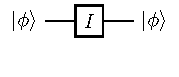
\includegraphics{images/3_Quantum_Computing/identity_gate.pdf}
    \caption{The schematic representation of the Identity gate}
\end{figure}

The NOT gate or $X$ gate is a quantum gate that operates on a single qubit. It tranforms
the qubit by swapping its amplitude coefficients. Let $\ket{\phi} = \phi_0\ket{0} + \phi_1\ket{1}$,
the the $X$ gate will tranform it as

\begin{equation}
    X\ket{\phi}=\begin{bmatrix}
        0 & 1\\
        1 & 0
    \end{bmatrix}
    \begin{bmatrix}
        \phi_0\\
        \phi_1
    \end{bmatrix}
    =
    \begin{bmatrix}
        0\cdot\phi_0 + 1\cdot\phi_1\\
        1\cdot\phi_0 + 0\cdot\phi_1
    \end{bmatrix}
    =
    \begin{bmatrix}
        \phi_1\\
        \phi_0
    \end{bmatrix}
\end{equation}

If the qubit $\ket{\phi}$ was either on state $\ket{0}$ or $\ket{1}$ this gate would
act as a logical negation - flipping the state of the qubit. For example, let
$\ket{\phi} = \ket{0} = 1\cdot\ket{0} + 0\cdot\ket{1}$ then

\begin{equation}
    X\ket{\phi} = 0\cdot\ket{1} + 1\cdot\ket{1} = \ket{1} = \ket{\phi'}
\end{equation}

The schematic representation of the $X$ gate is

\begin{figure}[ht]
    \centering
    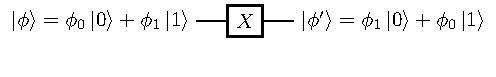
\includegraphics{images/3_Quantum_Computing/x_gate.pdf}
    \caption{The schematic representation of the $X$ gate}
\end{figure}

\begin{figure}[ht]
    \centering
    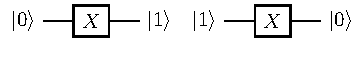
\includegraphics{images/3_Quantum_Computing/x_gate_ex1.pdf}
    \caption{The $X$ gate actions when the input qubit is at the $\ket{0}$ and $\ket{1}$ state respectively}
\end{figure}

The Hadamard gate is a quantum gate that operates on single qubits. It tranforms the qubit by
putting it on a superposition of its basis states. In matrix notation is represented as

\begin{equation}
    H=\frac{1}{\sqrt{2}}\begin{bmatrix}
        1 & 1\\
        1 & -1
    \end{bmatrix}
\end{equation}

Let a single qubit $\ket{\phi}$ have the computation basis $\ket{0},\ket{1}$, then
$\ket{\phi}=\phi_0\ket{0}+\phi_1\ket{1}$. The Hadamard gate will tranform it as

\begin{equation}
    H\ket{\phi}=\frac{1}{\sqrt{2}}\begin{bmatrix}
        1 & 1\\
        1 & -1\\
    \end{bmatrix}
    \begin{bmatrix}
        \phi_0\\
        \phi_1
    \end{bmatrix}
    =\frac{1}{\sqrt{2}}
    \begin{bmatrix}
        1\cdot\phi_0+1\cdot\phi_1\\
        1\cdot\phi_0-1\cdot\phi_1\\
    \end{bmatrix}
    =\frac{1}{\sqrt{2}}[
        (\phi_0+\phi_1)\ket{0}+
        (\phi_0-\phi_1)\ket{1}
    ]
\end{equation}

The schematic representation of the Hadamard gate is

\begin{figure}[ht]
    \centering
    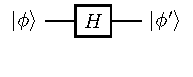
\includegraphics{images/3_Quantum_Computing/hadamard_gate.pdf}
    \caption{The schematic representation of the Hadamard gate}
\end{figure}

We can analyze further by assigning $\ket{\phi}$ to be on the two computation basis states:

\begin{enumerate}
    \item for $\ket{\phi} = \ket{0}$:
    \begin{equation}
        H\ket{\phi}=H\ket{0}=
        H(1\ket{0}+0\ket{1})=
        \frac{1}{\sqrt{2}}[(1+0)\ket{0}+(1-0)\ket{1}]=
        \frac{1}{\sqrt{2}}(\ket{0}+\ket{1})=\ket{+}
    \end{equation}
    \begin{figure}[ht]
        \centering
        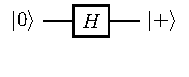
\includegraphics{images/3_Quantum_Computing/hadamard_gate_basis0.pdf}
        \caption{The tranformation of the $\ket{0}$ state to the $\ket{+}$ state}
    \end{figure}
    \item for $\ket{\phi} = \ket{1}$:
    \begin{equation}
        H\ket{\phi}=H\ket{1}=
        H(0\ket{0}+1\ket{1})=
        \frac{1}{\sqrt{2}}[(0+1)\ket{0}+(0-1)\ket{1}]=
        \frac{1}{\sqrt{2}}(\ket{0}-\ket{1})=\ket{-}
    \end{equation}
    \begin{figure}[ht]
        \centering
        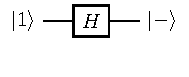
\includegraphics{images/3_Quantum_Computing/hadamard_gate_basis1.pdf}
        \caption{The tranformation of the $\ket{1}$ state to the $\ket{-}$ state}
    \end{figure}
\end{enumerate}

\subsection{Multi-Qubit Gates}

The Controlled-NOT gate or $CX$ gate is a quantum gate that operates on two qubits.
This gate operates by having a \textit{control} and \textit{target} qubit. If
the control qubit is on the $\ket{1}$ state then the target qubit is tranformed
by an $X$ gate tranformation - practically flipping its basis state. In matrix
notation is represented as

\begin{equation}
    CX=\begin{bmatrix}
        1 & 0 & 0 & 0 \\
        0 & 1 & 0 & 0 \\
        0 & 0 & 0 & 1 \\
        0 & 0 & 1 & 0 \\
    \end{bmatrix}
\end{equation}

Let $\ket{\phi}$ be a quantum register of two qubits $\ket{x},\ket{y}$. Then
$\ket{\phi}=\ket{x\otimes y}=\ket{xy}$. We shall note the matrix and linear notation
of the quantum register is

\begin{equation}
    \ket{\phi}=
    \begin{bmatrix}
        x_0y_0\\
        x_0y_1\\
        x_1y_0\\
        x_1y_1
    \end{bmatrix}=
    \begin{bmatrix}
        \phi_0\\
        \phi_1\\
        \phi_2\\
        \phi_3
    \end{bmatrix}=
    \phi_0\ket{00}+\phi_1\ket{01}+\phi_2\ket{10}+\phi_3\ket{11}
\end{equation}

The $CX$ gate will act upon $\ket{\phi}$ as follows

\begin{equation}
    CX\ket{\phi}=\begin{bmatrix}
        1 & 0 & 0 & 0 \\
        0 & 1 & 0 & 0 \\
        0 & 0 & 0 & 1 \\
        0 & 0 & 1 & 0
    \end{bmatrix}
    \begin{bmatrix}
        \phi_0 \\
        \phi_1 \\
        \phi_2 \\
        \phi_3
    \end{bmatrix}=
    \begin{bmatrix}
        \phi_0 \\
        \phi_1 \\
        \phi_3 \\
        \phi_2
    \end{bmatrix}=
    \phi_0\ket{00}+\phi_1\ket{01}+\phi_3\ket{10}+\phi_2\ket{11}
\end{equation}

The schematic representation of the $CX$ gate is
\begin{figure}[ht]
    \centering
    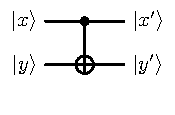
\includegraphics{images/3_Quantum_Computing/cx_gate.pdf}
    \caption{The schematic representation of the $CX$ gate}
\end{figure}

Lastly we will discuss the Controlled-CX gate or $CCX$ gate. The $CCX$ gate is quantum
gate that operates on three qubits. This gate is similar to the $CX$ gate but instead
of having only one control qubit it has two. In matrix notation is represented as

\begin{equation}
    CCX=\begin{bmatrix}
        1 & 0 & 0 & 0 & 0 & 0 & 0 & 0 \\
        0 & 1 & 0 & 0 & 0 & 0 & 0 & 0 \\
        0 & 0 & 1 & 0 & 0 & 0 & 0 & 0 \\
        0 & 0 & 0 & 1 & 0 & 0 & 0 & 0 \\
        0 & 0 & 0 & 0 & 1 & 0 & 0 & 0 \\
        0 & 0 & 0 & 0 & 0 & 1 & 0 & 0 \\
        0 & 0 & 0 & 0 & 0 & 0 & 0 & 1 \\
        0 & 0 & 0 & 0 & 0 & 0 & 1 & 0 \\
    \end{bmatrix}
\end{equation}

Let $\ket{\phi}$ be a quantum register of three qubits $\ket{x},\ket{y},\ket{z}$. Then
$\ket{\phi}=\ket{x\otimes y\otimes z}=\ket{xyz}$. We shall note the matrix and linear notation
of the quantum register is

\begin{equation}
    \ket{\phi}=
    \begin{bmatrix}
        x_0y_0z_0\\
        x_0y_0z_1\\
        x_0y_1z_0\\
        x_0y_1z_1\\
        x_1y_0z_0\\
        x_1y_0z_1\\
        x_1y_1z_0\\
        x_1y_1z_1\\
    \end{bmatrix}=
    \begin{bmatrix}
        \phi_0\\
        \phi_1\\
        \phi_2\\
        \phi_3\\
        \phi_4\\
        \phi_5\\
        \phi_6\\
        \phi_7
    \end{bmatrix}=
    \phi_0\ket{000}+\phi_1\ket{001}+\phi_2\ket{010}+\phi_3\ket{011}+\phi_4\ket{100}+\phi_5\ket{101}+\phi_6\ket{110}+\phi_7\ket{111}
\end{equation}

The $CCX$ gate will act upon $\ket{\phi}$ as follows

\begin{equation}
    CCX\ket{\phi}=\begin{bmatrix}
        1 & 0 & \hdots & 0 & 0 \\
        0 & 1 & \hdots & 0 & 0 \\
        \vdots & \vdots & \ddots & \vdots & \vdots \\
        0 & 0 & \hdots & 0 & 1 \\
        0 & 0 & \hdots & 1 & 0 \\
    \end{bmatrix}
    \begin{bmatrix}
        \phi_0\\
        \phi_1\\
        \vdots \\
        \phi_6\\
        \phi_7
    \end{bmatrix}=
    \begin{bmatrix}
        \phi_0\\
        \phi_1\\
        \vdots \\
        \phi_7\\
        \phi_6
    \end{bmatrix}=
    \phi_0\ket{000}+\phi_1\ket{001}+\hdots+\phi_7\ket{110}+\phi_6\ket{111}
\end{equation}

The schematic representation of the $CCX$ gate is

\begin{figure}[ht]
    \centering
    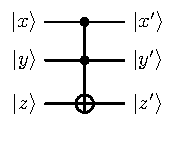
\includegraphics{images/3_Quantum_Computing/ccx_gate.pdf}
    \caption{The schematic representation of the $CCX$ gate}
\end{figure}